\documentclass{article}
\usepackage{listings}
\usepackage{enumitem}
\usepackage[cachedir=minted_cache]{minted}
\usepackage{graphicx}
\graphicspath{ {./img/} }
\usepackage[margin=1in]{geometry} %used to set the margins
\setcounter{secnumdepth}{0} %used to get rid of section numbers
\title{Lab 2}
\author{Michael Morikawa \& James Daza}
\date{\today}


\begin{document}
    \maketitle
    \section{Lab Questions}
    \begin{enumerate}[label=\textbf{Question \arabic*}]
        \item What are some effective techniques to generate an integer value 
        for a key of data type string?\\
        \textbf{
            Polynomial hashing and cyclic shift are the most effective.
        }
        \item Whate are some examples of compression functions? \\
        \textbf{Division} $f(x)\%N$ \textbf{MAD: }$(a \cdot f(x) + b)\%N)$
    \end{enumerate}

    \section{Source Code}
    \inputminted{c++}{../src/main.cpp}

    \section{Output}
    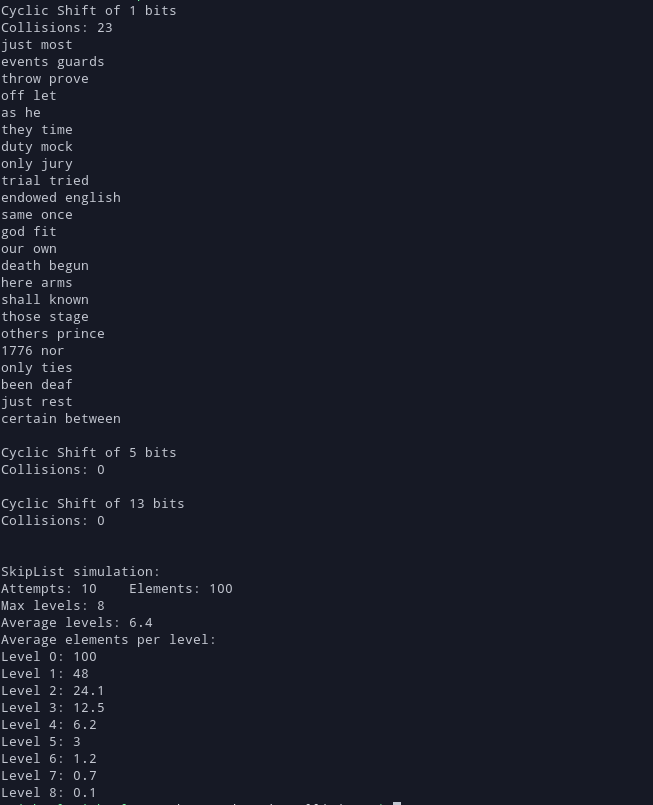
\includegraphics[scale=0.7]{lab2_output.png}


\end{document}